% !TEX root = ../main.tex

\chapter{Technical execution} % (fold)
\label{chp:execution}

\section{Organising state} % (fold)
\label{sec:organising_state}

talk about the difference between storing params and storing widgets

% section organising_state (end)

\section{Changing terminology} % (fold)
\label{sec:changing_terminology}

Terminology now is the same as in the API

Users don't understand the difference between facet and filter

Make a higher-level language that only uses filters

Mention the doc changes needed

% section changing_terminology (end)

\section{Handling state changes} % (fold)
\label{sec:handling_state_changes}

Research:

\begin{itemize}
  \item observables vs flux
  \item Other languages (Elm model)\cite{csstricks-elm}
\end{itemize}

% section handling_state_changes (end)

\section{Getting responses from the API} % (fold)
\label{sec:getting_responses_from_the_api}

another function listens to changes in state

it transforms params into a JS client request

it replaces the {\tt response} in the state with an action

% section getting_responses_from_the_api (end)

\section{Rendering refinements} % (fold)
\label{sec:rendering_refinements}

Stuff to think about: dynamic facets as core part of this API or not?

% section rendering_refinements (end)

\section{Saved state} % (fold)
\label{sec:saved_state}

allow for replacing of whole state

reasons

\begin{enumerate}
  \item saving state in url
  \item saving state in localstorage
  \item SSR
\end{enumerate}

documentation very clear that this shouldn't regularly be used

% section saved_state (end)

\section{Overview} % (fold)
\label{sec:overview}

\begin{figure}[H]
\label{figure:core-architecture}
  \centering
  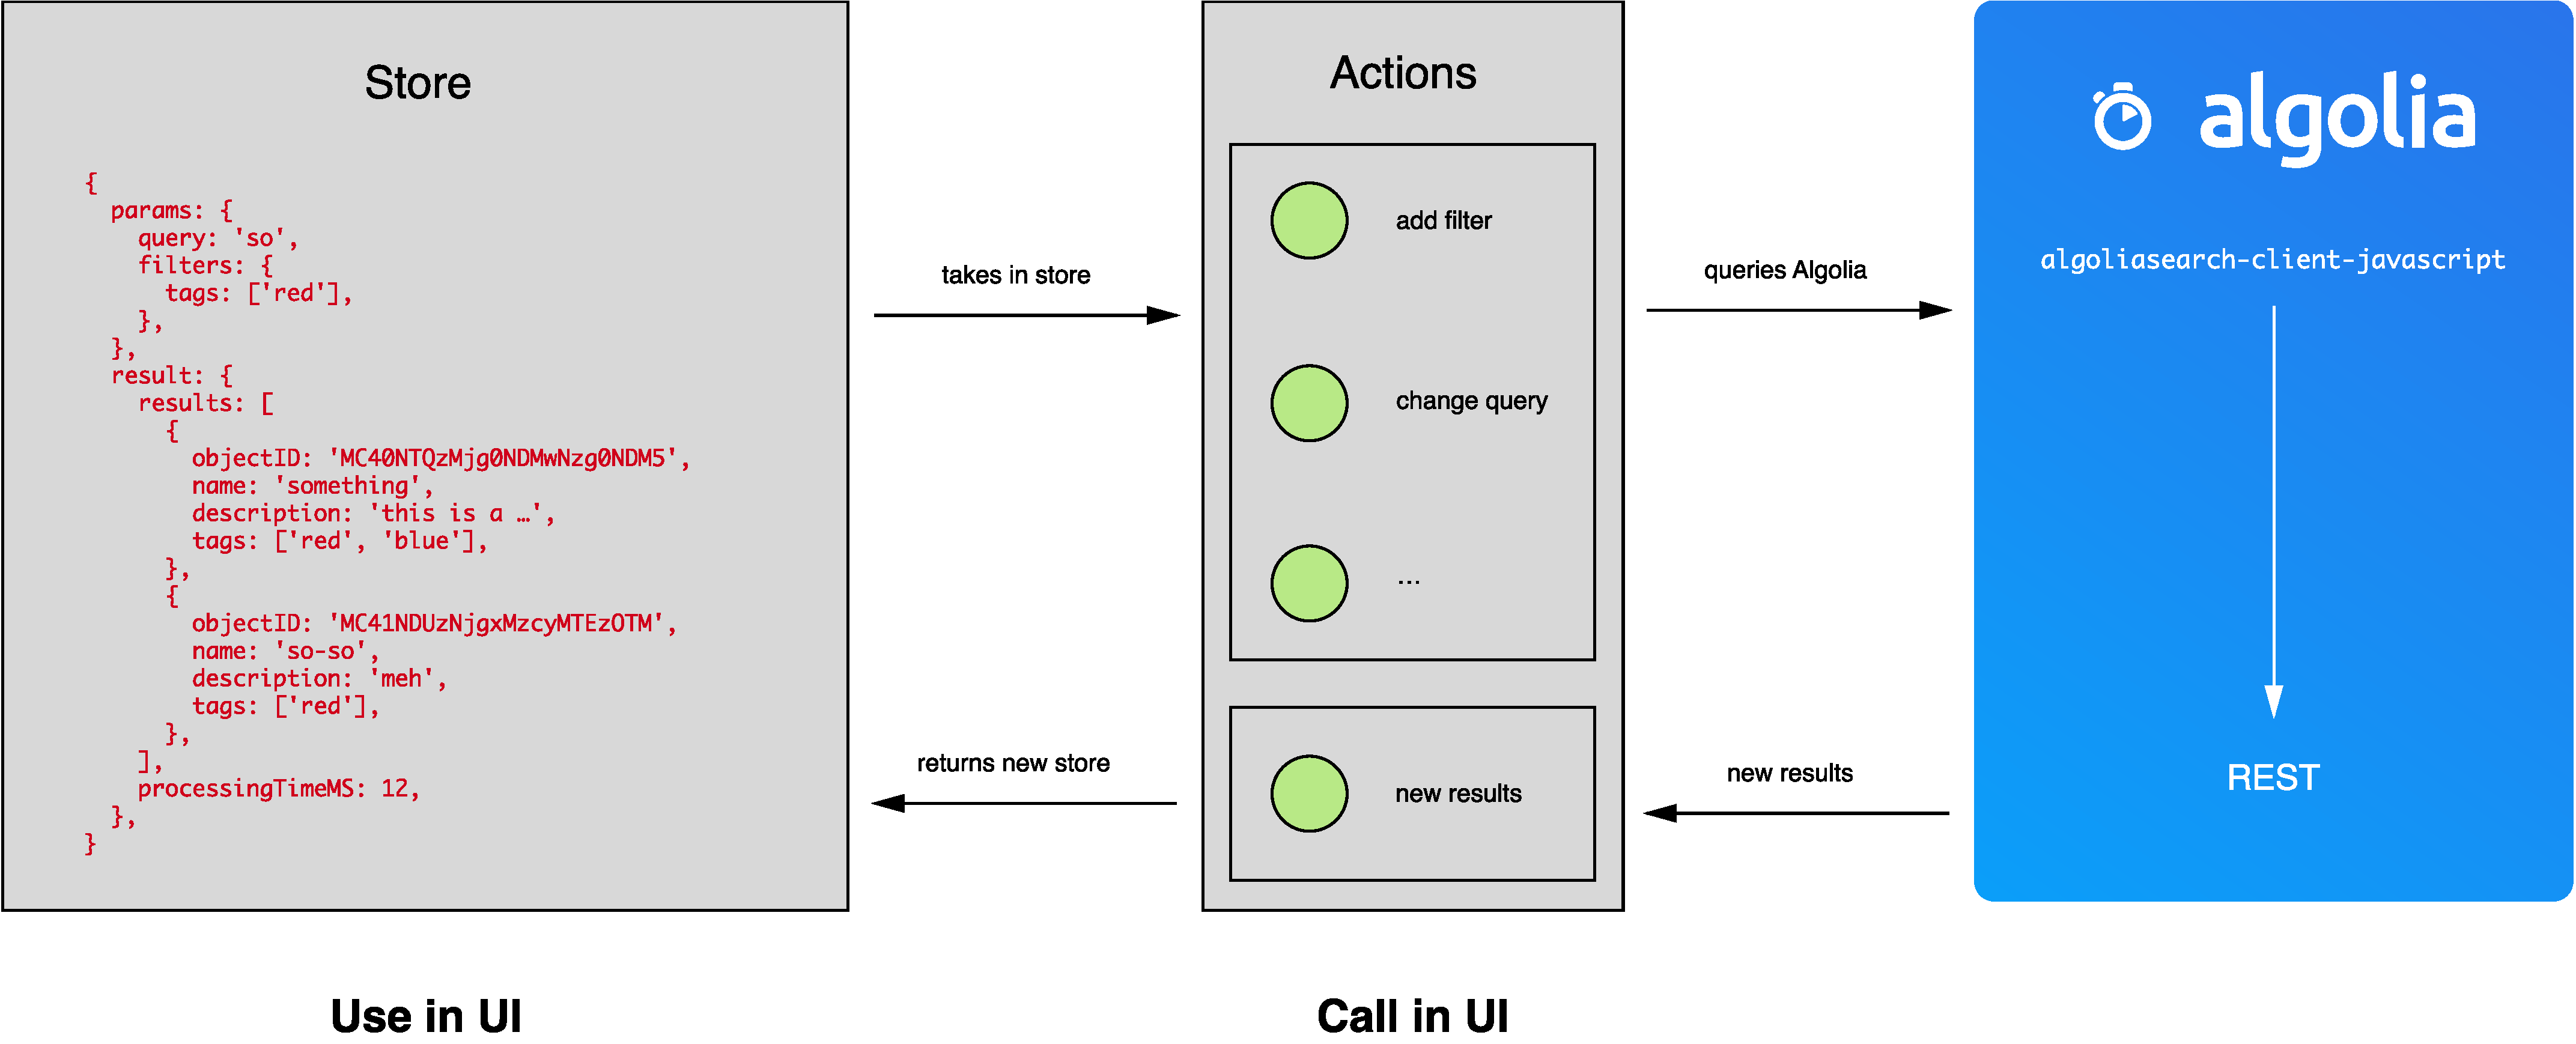
\includegraphics[width=\textwidth]{../assets/architecture.pdf}
  \caption{Architecture overview\cite{blog-architecture}}
\end{figure}

% section overview (end)

\section{Complete implementation} % (fold)
\label{sec:complete_implementation}

Obviously this isn't final and too detailed.

\begin{lstlisting}[caption={Using instantearch-core},label={lst:is-core-usage}]
// stores.js
import algoliasearch from 'algoliasearch';
import { createStore } from 'instantsearch-core';

const appId = 'OFCNCOG2CU';
const apiKey = 'f54e21fa3a2a0160595bb058179bfb1e';
const indexName = 'products_asc';

const client = algoliasearch(appId, apiKey);
const productsStore = createStore(client, indexName);

export productsStore;

// widget.js
import { setQuery } from 'instantsearch-core/actions/query';
import { productsStore } from './stores';

function onInput(event) {
  event.preventDefault();

  productsStore.refine(setQuery(event.target.value));
}
\end{lstlisting}

% section complete_implementation (end)

